\documentclass[12pt]{article}
\usepackage{indentfirst}
\usepackage{siunitx}
\usepackage{graphicx}
\usepackage{subfigure}
\usepackage{float}
\usepackage{amsmath}
\usepackage{tikz}
\usepackage{pgfplots}
\usepackage{enumitem}
\usepackage[utf8]{inputenc}
\usepackage{enumerate}


\setlength{\parindent}{20pt}
\setlength{\oddsidemargin}{1cm}
\setlength{\evensidemargin}{1cm}
\setlength{\marginparsep}{0.5cm}
\setlength{\marginparwidth}{1.5cm}
\setlength{\textwidth}{150mm}
\renewcommand{\baselinestretch}{1.25}

\begin{document}
	
	\begin{titlepage}
		\vspace*{\stretch{-0.7}}
		\begin{center}
			\Large{Emergency Supplies Management: An Integrated Model for Deployment of Transport UAV}\\
			\Large{Control \#1908684}\\
			\textit{January 29, 2019}\\
			~\\
			\textbf{Abstract} 
		\end{center}
		The hurricane Maria hit Puerto Rico in 2017 and created great damages on the island. To help the government with disaster assistance, HELP, Inc. is attempting to send a drone fleet to the affected area. The fleet will be able to perform two missions—medical supply and video reconnaissance. This paper tries to make a detailed plan for HELP, Inc. to conduct this disaster operation, including drone fleet configuration and flight route plan. Careful analysis implies that the problem is similar to the Vehicle Routing Problem (VRP) and the Traveling Salesman Problem (TSP). Current studies give solutions to these problems only when most of the needed conditions are determined, for example, where the vehicles leave or what set of cargo is needed to transport. However, most of the things needed to make a plan remain unknown in this problem. Therefore, what kind of set of drones and medical packages to choose, where to launch them and the how to make a flight plan rely on each other. We found an appropriate solution has not been provided by current studies yet. In view of these difficulties, we take the specification of cargoes and their relationship with selection of drones into consideration. We utilized the specifications of cargoes and applied optimization methods in an integrated approach. Our model also considered the decrease of drones' flight time while carrying cargoes. The results shows that the model we proposed can provide 89 days medical supports in maximum. It provides a highly optimized plan for HELP, Inc.
		\vspace*{\stretch{1}}
	\end{titlepage}
	
	\tableofcontents
	\newpage
	
	\section{Introduction}
	
		\subsection{Background}
		In 2017, the hurricane Maria to ever hit the United States territory of Puerto Rico left the island with severe damage and caused over 2900 fatalities. Aiming to fill the gap of medical supplies after the disaster and help locals to restore the infrastructures, a non-governmental organizations is attempting to design a transportable disaster response system to handle similar scenarios in the future. The function of the disaster response system consists of two aspects: (a) delivery of required medical packages to medical centers located in different cities, (b) reconnaissance of main roads affected by hurricane. The disaster response system is expected to utilize a fleet of UAV(Unmanned aerial vehicle) to deliver medical supplies to specific cities and provide high-resolution video of transportable road networks to remote control center. \par 
		Based on given requirements and information, we designed a transportation model targeted to similar scenarios. In this paper, we will focus on three optimizations: (1) drone payload configuration, (2) ISO container configuration, (3) locations of the containers. \par 
		
		\subsection{Outline of Our Approach}
		The beginning of our paper will focus on developing the necessary framework for modeling. We will first summarize the geometric features of medical packages and drones' payload. Then we will introduce the route scheduling and packaging algorithms we used for a container in a fixed location. \par 
		The second part will analyze the actual scenario in Puerto Rico, that is, we will define a criterion to describe the degree of emergency for affected cities by the geographical information of the hurricane and city locations. The criterion will be involved in weighting our value functions. In last we will illustrate our searching strategy in finding the best three locations for containers using the criterion defined before.\par 
		Our model will be illustrated by detailed mathematical descriptions in part three. We will perform a simulation with respect to constraints and searching algorithms we proposed and discuss the result we collected from computer simulations.\par 
		In the end of our paper we will give our answers to the three problems above, and compare the actual scenario with the expected result of our model, in order to further evaluate the compatibility of our model. \par    
		
		\subsection{Preliminary Assumptions}
		Due to the fact that the function of the response system consists of two different parts and actual situation is much more complicated than expectation, we will introduce a few preliminary assumptions to our model.
		\begin{itemize}
			\item Weather conditions of the island is approximately static during the response system being enabled 
			\item The priority of transporting medical packages is \textit{higher} than the priority of road reconnaissance
			\item Extra medical packages can be stored in the local medical centers 
			\item Multiple drones can fly through the same route at the same time without conflicting with each other
			\item Altitude of different regions will not affect the route and performance of drones
			\item Drones can return back to container after finish one delivery, and start another delivery if it has sufficient battery power
			\item Edges of cargoes in cargo bay must be aligned to the parallel lines of the container wall
			\item Drone tethers are not suitable in this system. The usage of a drone tether is to charge the drones and fix them in the air, but due to its short length, the general scenarios which require a drone tether is to use the drone as a communication base station. In our case, the objectives of drones are to transport medical packages and provide video of main roads, which means it is not necessary to carry a tether with them in the container. 
			\item Drone A has the smallest payload and maximum flight distance but does not have the smallest size among all types of drone in list. Thus we exclude drone A from our consideration in following optimizations. 
			\item Med packages can be embedded in cargo bays to reduce space occupation when the cargo bays are packed in the containers
		\end{itemize}

		\subsection{Constraints of Cargo Container}
			Assume that we are dealing with a set of $k$ cargoes, $C = \{c_i \mid 1 \leq i \leq k\}$, in which $i$th cargo has length $l$, width $w$ and height $h$. Each cargo has 6 possible ways to be placed in the container by
			\begin{figure}[H]
				\centering
				\subfigure{}{
					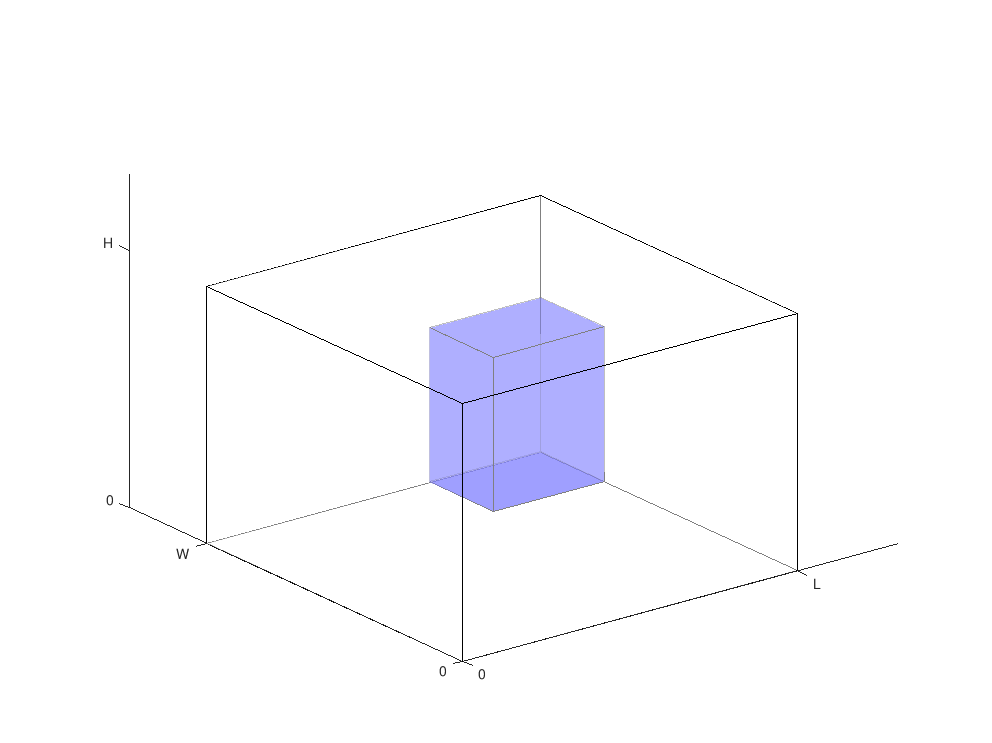
\includegraphics[width=0.28\textwidth, height=0.25\linewidth]{/home/vitowu/Documents/CourseMaterials/CourseMaterials/2018-2019_Term2/2019MCM-ProblemB/paper/cargo_1.png}
					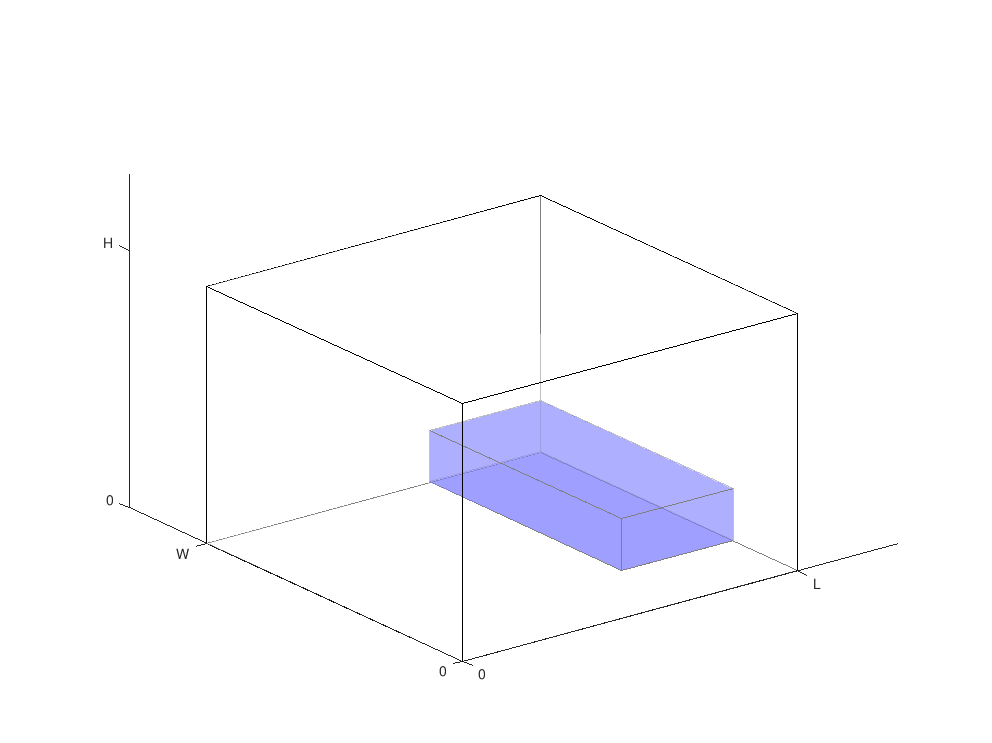
\includegraphics[width=0.28\textwidth, height=0.25\linewidth]{/home/vitowu/Documents/CourseMaterials/CourseMaterials/2018-2019_Term2/2019MCM-ProblemB/paper/cargo_2.png}
					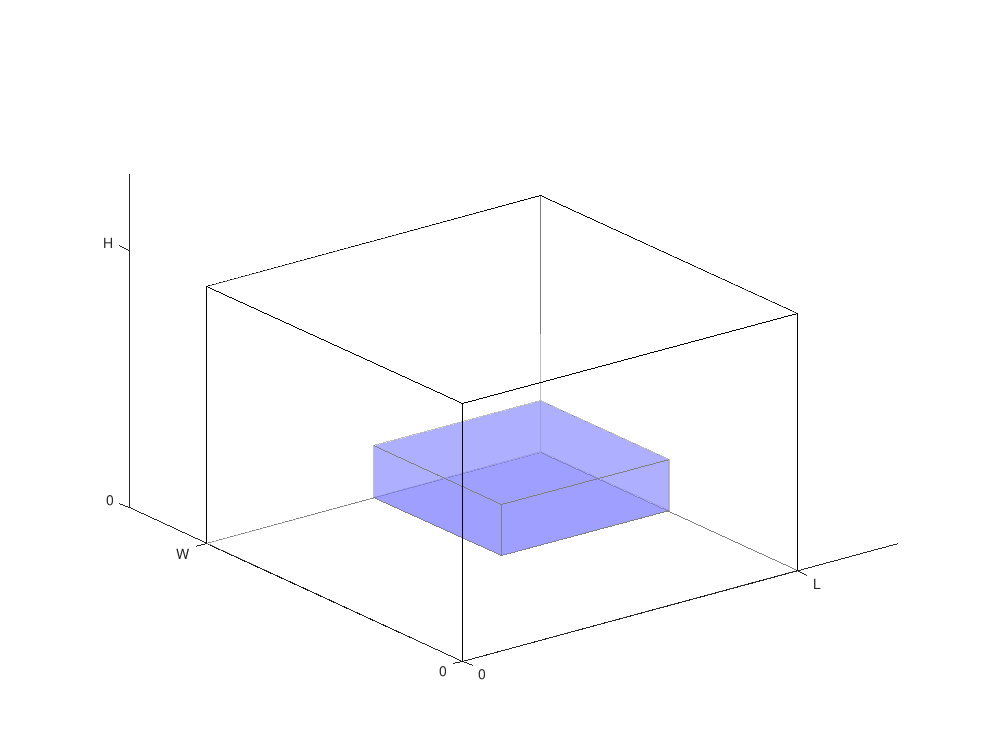
\includegraphics[width=0.28\textwidth, height=0.25\linewidth]{/home/vitowu/Documents/CourseMaterials/CourseMaterials/2018-2019_Term2/2019MCM-ProblemB/paper/cargo_3.png}
					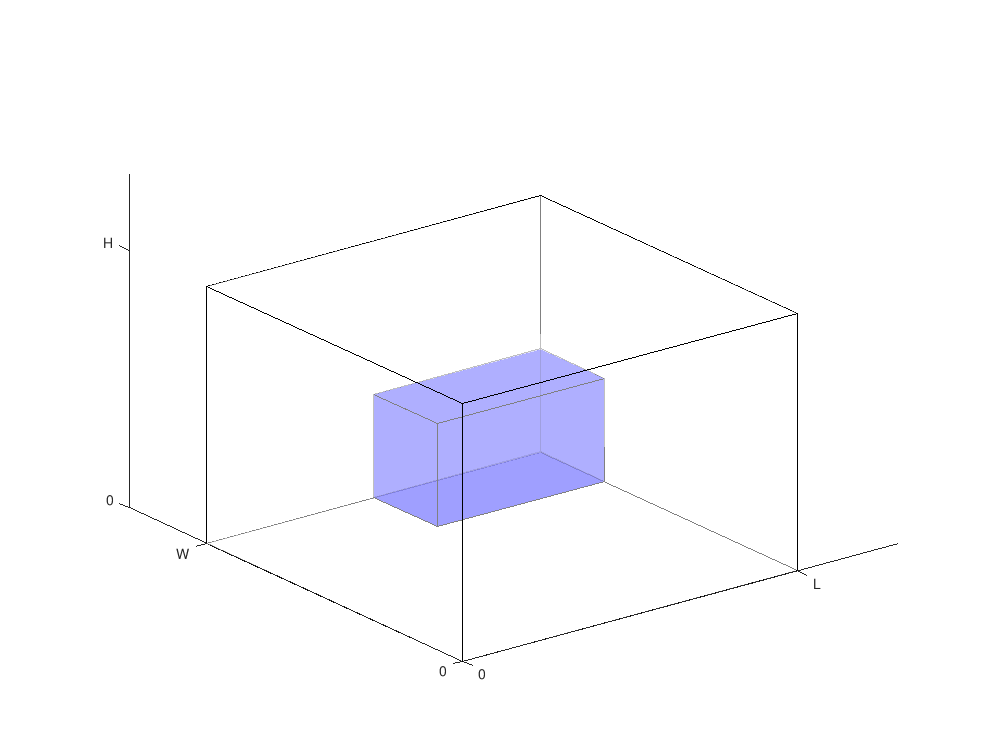
\includegraphics[width=0.28\textwidth, height=0.25\linewidth]{/home/vitowu/Documents/CourseMaterials/CourseMaterials/2018-2019_Term2/2019MCM-ProblemB/paper/cargo_4.png}
					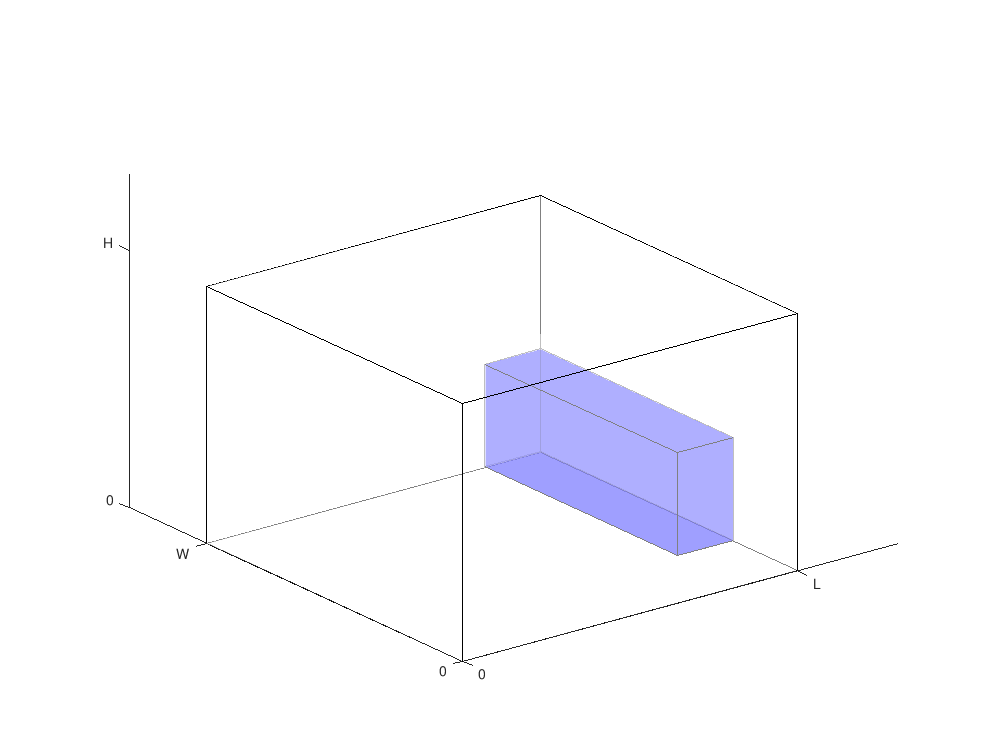
\includegraphics[width=0.28\textwidth, height=0.25\linewidth]{/home/vitowu/Documents/CourseMaterials/CourseMaterials/2018-2019_Term2/2019MCM-ProblemB/paper/cargo_5.png}
					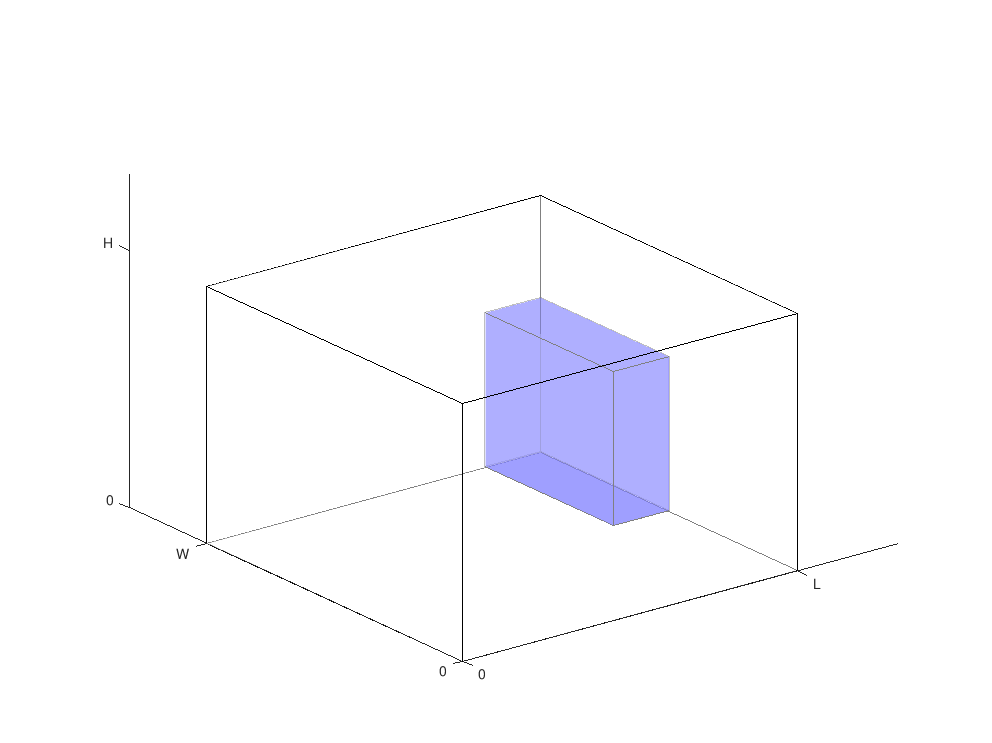
\includegraphics[width=0.28\textwidth, height=0.25\linewidth]{/home/vitowu/Documents/CourseMaterials/CourseMaterials/2018-2019_Term2/2019MCM-ProblemB/paper/cargo_6.png}
				}
			\end{figure}
			\par  
			Use ($l_i$,$w_i$,$h_i$) to denote the length of edges of $c_i$ that are parallel to L axis, W axis and H axis respectively. As shown in the figure, for different ways of placing the cargo $c_i$, ($l_i$,$w_i$,$h_i$) will be different (i.e. ($l$,$w$,$h$), ($l$,$h$,$w$), ($w$,$l$,$h$), ($w$,$h$,$l$), ($h$,$l$,$w$) or ($h$,$w$,$l$)). Now for a container $\tilde{P}$ with length $\tilde{L}$, width $\tilde{W}$ and height $\tilde{H}$, $\forall c_i, c_j \in C$ should follow the constraints
			\begin{equation}
				\left\{
					\begin{array}{lr}
						\frac{1}{2}l_i \leq a_i \leq \tilde{L} - \frac{1}{2}l_i, & \frac{1}{2}(l_i+l_j) \leq \mid a_i - a_j \mid \leq \tilde{L} - \frac{1}{2}(l_i+l_j)\\
						\frac{1}{2}w_i \leq b_i \leq \tilde{W} - \frac{1}{2}w_i, & \frac{1}{2}(w_i+w_j) \leq \mid b_i - b_j \mid \leq \tilde{W} - \frac{1}{2}(w_i+w_j)\\
						\frac{1}{2}h_i \leq b_i \leq \tilde{H} - \frac{1}{2}h_i, & \frac{1}{2}(h_i+h_j) \leq \mid c_i - c_j \mid \leq \tilde{H} - \frac{1}{2}(h_i+h_j)\\
					\end{array}
				\right.
			\end{equation}
			where $(a, b, c)$ is the coordinate of cargo $c$'s geometric center. \\
			~\\
			\textbf{Invarient of Cargo Bay Type 2}\par 
			An obvious invarient of given medical package configurations is that: \textit{MED-1} has the largest length, width and height among all MEDs. After calculation, cargo bay type 2 is capable to accommodate 15 \textit{MED-1} in maximum, which weights 30(lbs.) in total. However, the drone with maximum payload can carry only 22(lbs.). Therefore, if the container can contain $x$ MED-1s, by substituting MED-1 with other MEDs, it is still able to fit the cargo bay type 2 in size.  Also, the other MEDs' weight is greater or equal to MED-1's weight. Thus the cargo can contain at least $x$ MEDs. Since MED-1 won't exceed the size restriction if it doesn't exceed the weight restriction, we conclude that the only constraint for cargo bay type 2 is is $\sum_{c\in C}weight(c) \leq payload$.    
		\subsection{Optimized Route Scheduling and Packaging}	
			\subsubsection{Clarke-Wright Saving Algorithm for Vehicle Routing}
			
			If the location of the container is fixed and the package configuration is determined, the efficiency of delivery depends only on the route we choose. For this problem, we apply saving algorithm to calculate the maximum \textit{value function} $S_{max}$ for a fixed location and package configuration. (note: value function will be illustrated in section 4) 
			
			\begin{tikzpicture}[shorten >=1pt,->]
			\tikzstyle{vertex}=[circle,fill=black!25,minimum size=12pt,inner sep=2pt]
			\node[vertex] (G_1) at (0,0)   {0};
			\node[vertex] (G_2) at (4,3)   {1};
			\node[vertex] (G_3) at (1, 2) {2};
			\node[vertex] (G_4) at (-5,2)  {3};
			\draw[<->] (G_1) -- node[auto]{$l_{01}$} (G_2);
			\draw[<->] (G_1) -- node[auto]{$l_{02}$} (G_3);
			\draw[<->] (G_1) -- node[auto]{$l_{03}$} (G_4);
			\draw[<->] (G_2) -- node[auto]{$l_{12}$} (G_3);
			\draw[<->] (G_2) -- node[auto]{$l_{13}$} (G_4);
			\draw[<->] (G_3) -- node[auto]{$l_{23}$} (G_4);
			\end{tikzpicture}
		
			For each drone in package configuration,\par
			\textbf{Step 1:} Calculate cost matrix $L = {l(i;j)}$, where $i,j = 0,...,n$, $n = \mid R\mid$ \par
			\textbf{Step 2:} Ordering the value-loss $l_{ij}$ from largest to smallest \par 
			\textbf{Step 3:} Start from the largest value-loss \par 
			\hspace{1.5cm}  \textbf{\textit{(a)}.} If linking medical center $i$ and $j$ results in a route with less value-loss, then add this link to the tour. If not, abort the link.\par 
			\hspace{1.5cm}  \textbf{\textit{(b)}.} Perform (a) in the new matrix until all distances of possible tours in the matrix are the maximum distance the drone can fly through. \par 
			\textbf{Step 4:} denote the terminated matrix as $\tilde{L}$ \par 
			\textbf{Step 5:} $S_{max} = S(\tilde{L})$ \par 
			 
			\subsubsection{Dynamic Programming for Cargo Selection}
			If the location of the container is fixed, the optimization on package configuration can then be simplified to a dynamic programming problem. The Bellman equation can be given by
			\begin{equation}
				Q(v_t) = \max Q(v_t+\zeta_i, x_i \mid S_{i_{max}})
			\end{equation}
			where $\zeta_i$ is the cost of $i$th objects. In this case, cost $\zeta$ is determined by the size of the object $i$. Variable $x$ represents whether a cargo is in the container
			\begin{equation}
			x = 
			\begin{cases}
			1 &\mbox{, if cargo is in the container} \\
			0 &\mbox{, otherwise}
			\end{cases}
			\end{equation}
			\par 
		
		\subsection{Scenario of Disaster}
			\subsubsection{Geography and Topography of Puerto Rico}
			From Monore, W.H.'s 1976 report of landforms of Puerto Rico (Monore, W.H., 1976) and another research group's plot of section view of Puerto Rico in 2001 (Ariel E. Lugo, et al., 2001), we can conclude that the central part of Puerto Rico is mountainous, and the area of north and northeast coast is flat lowlands. 
			\begin{figure}[H]
				\centering
				\subfigure{}{
					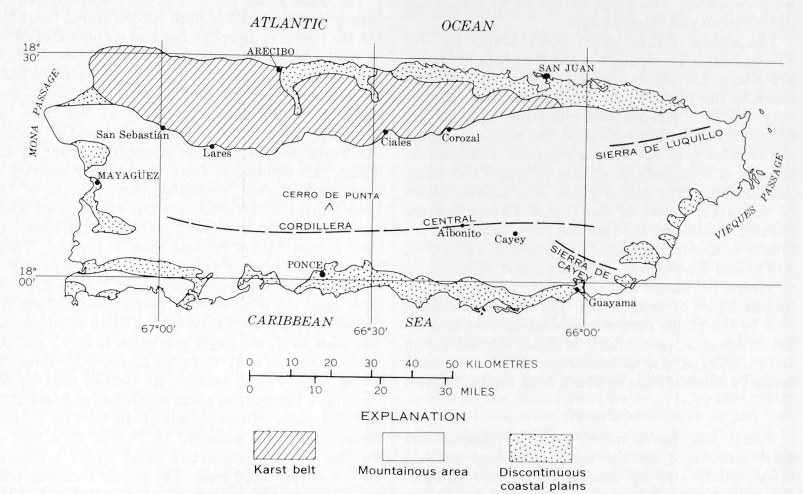
\includegraphics[width=0.5\textwidth, ]{/home/vitowu/Documents/CourseMaterials/CourseMaterials/2018-2019_Term2/2019MCM-ProblemB/paper/Puerto_Rico_Topography.png}
				}
				\subfigure{}{
					
\includegraphics[width=0.45\textwidth,height=0.3\linewidth ]{/home/vitowu/Documents/CourseMaterials/CourseMaterials/2018-2019_Term2/2019MCM-ProblemB/paper/Puerto_Rico_Section_View.png}
				}
			\end{figure}
			From the observation one intuition can be inferred that the hurricane had much significant impacts on north coast of Puerto Rico compared with the central part and the south part. Also, it is reasonable to infer that the infrastructures are mostly located in the north coast of Puerto Rico. 
			
			\subsubsection{Hurricane Maria}
			\begin{figure}[H]
				\centering
				\subfigure{}{
					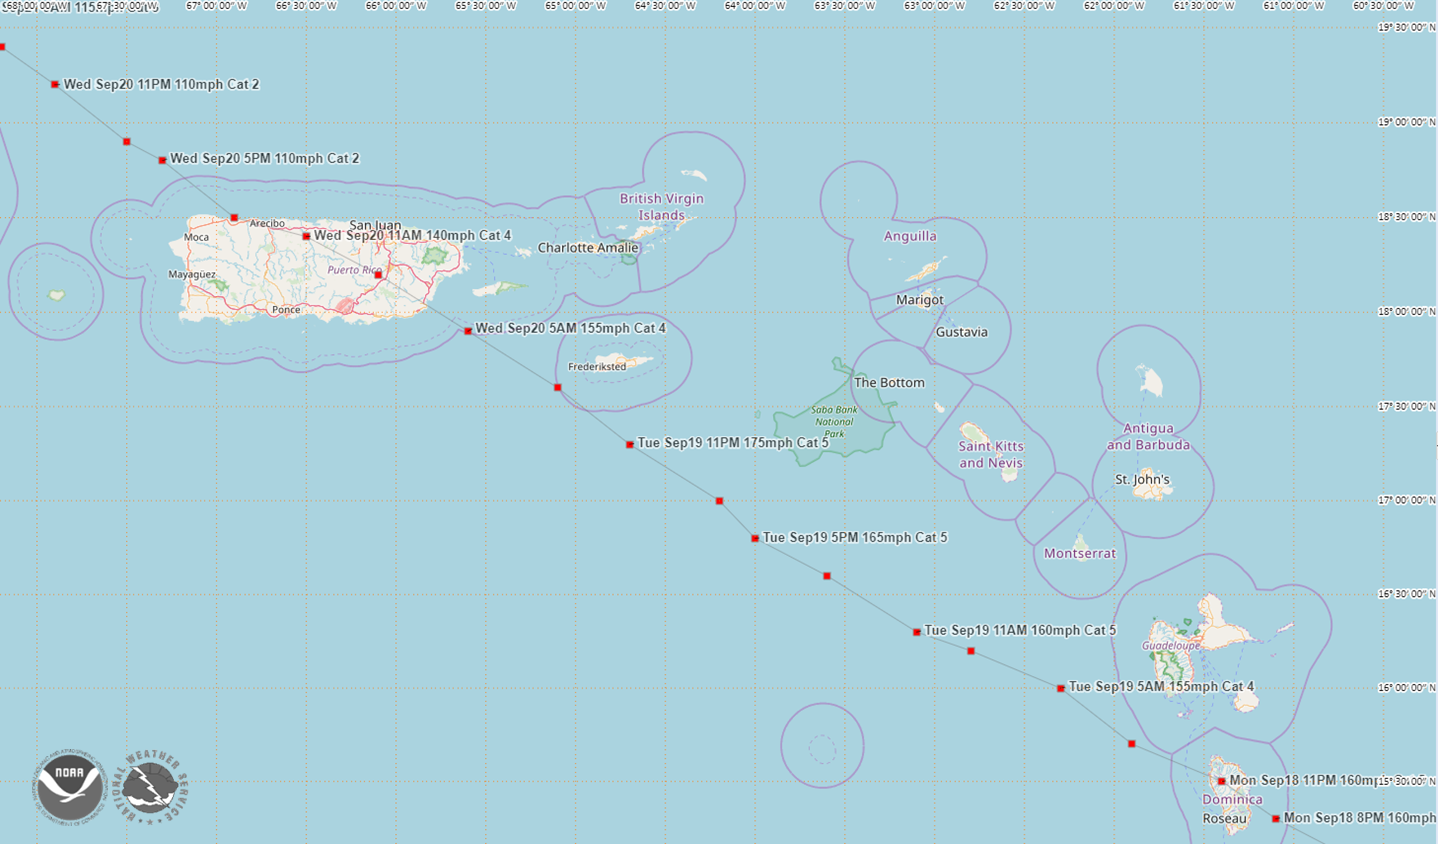
\includegraphics[width=0.5\textwidth, ]{/home/vitowu/Documents/CourseMaterials/CourseMaterials/2018-2019_Term2/2019MCM-ProblemB/paper/MariaTrack.PNG}
				}
				\subfigure{}{
					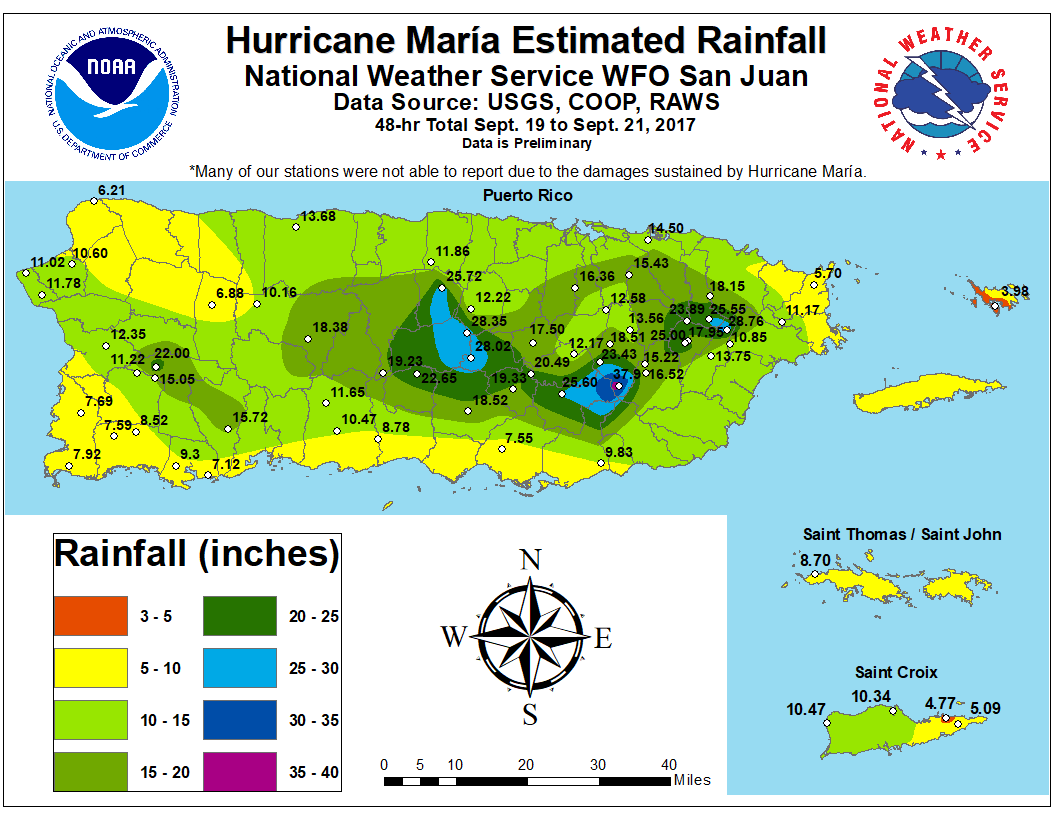
\includegraphics[width=0.45\textwidth,height=0.3\linewidth ]{/home/vitowu/Documents/CourseMaterials/CourseMaterials/2018-2019_Term2/2019MCM-ProblemB/paper/Maria_Rainfall.png}
				}
			\end{figure}
			At Sept. 20th 2017, Hurricane Maria landed at the southeast coast of Puerto Rico, and then crossed through the island towards northwest. The trace of hurricane can be given by statistics of meteorological satellites.
			
			\subsubsection{Degree of Emergency \textit{$\lambda$}}
			Since that the degree of damage for cities in different geographical locations are mutually distinct, a criterion to describe the degree of emergency is necessary to be purposed in order to meet the actual scenarios.\par 
			The degree of emergency $\lambda$ in our model is given by
			\begin{equation}
				\lambda(m_i) = (1 + \frac{cos \tilde{\theta} * Latitude(m_i)}{\alpha}) T
			\end{equation}
			where $m_i$ denotes the $i$th medical center, $T$ is the expected number of days, $\alpha$ is a calibration coefficient and $\tilde{\theta}$ is the angle between the trace of hurricane and North-South line.
			
		\subsection{Search Locations to Place Containers}
		Now that we have designed approaches to determine the package configuration and delivery route for containers in fixed location in optimal, we can then search 3 coordinates globally in the map of Puerto Rico to allocate 3 containers. \par
		To reduce the complexity of calculation, following strategies will be applied in searching process
		\begin{itemize}
			\item The searching area is where the nearest medical center is within 50km, since the priority of delivery is higher than the priority of road reconnaissance, .
			\item Searching area will exclude areas with latitude smaller than 18.215 because our targeted medical centers are integrated in the north part of Puerto Rico.
			\item The distance between two containers should larger than 10km due to the consideration of fairness. Placing two containers with a short distance between will not be a efficient strategy.
		\end{itemize} 

	\section{Modeling of Delivery}
		\subsection{Definition of Values}
			\begin{table}[H]
				\centering
				\begin{tabular}{c c}
					\hline\hline
					$l_i$ & length of cargo $i$ \\ 
					$w_i$ & width of cargo $i$  \\
					$h_i$ & height of cargo $i$ \\ 
					$K(w, l, h)$ & constraints of width, height and length \\
					$\omega_i$ & weight of cargo $i$ \\
					$\tilde{T}(m_j)$ & \begin{tabular}{@{}c@{}}number of days for city $j$ \\ which have medical support from the system\end{tabular} \\ 
					$\lambda(m_j)$ & city $j$'s degree of emergency \\
					$\tilde{G_k}$ & maximum flight time of drone without carrying cargoes $k$ \\
					$\tilde{Y_k}$ & speed of drone $k$ \\
					$\tilde{p_k}$ & maximum payload of drone $p$ \\ 
					\hline
				\end{tabular}
			\end{table}
			
		\subsection{Definition of Functions}
		
			\subsubsection{Flight Time Inequality}	
			The flight time of a drone depends on its maximum flight time without carrying cargoes and the its payload during the actual flight. The total flight time of the drone will follow the \textit{flight time inequality}
			\begin{equation}
			\sum_{i=0}^{N}[\frac{(N-i)p_i}{\tilde{p_k}}]^{\beta_k} \leq 1
			\end{equation}	
			Here, $N$ is the total number of flight routes in which the drone has different payloads, $p_i$ is the payload in $i$th flight route and $\beta_k$ is the impact factor of payload onto the decrease of flight time.
			
			\subsubsection{Local Value Function \textit{S}}
			To better evaluate the actual effect of a container which had been packaged with a set of cargoes and located in a fixed location, we introduce a local value function \textit{S} to describe the local value. \par 
			\begin{equation}
				S(L) = \frac{1}{2}\sum_{m \in \mathcal{M}}\frac{\lambda(m)\tilde{T}(m)}{{\mid}\mathcal{M}{\mid}} + \frac{\sum_{m\in\mathcal{M}}(\tilde{T}(m)-\bar{\tilde{T}})^2}{{\mid}\mathcal{M}{\mid}}
			\end{equation}
			in which we use $\mathcal{M}$ to denote the set of medical centers involved in distance matrix $L$.  \par 
			The first term of $S$ is the average number of days for each medical center in $L$, weighting with the degree of emergency $\lambda(m)$ respectively, and the second term is aiming to evaluate the degree of fairness in order to avoid unbalanced deliveries. 
			
			\subsubsection{Bellman Equation and Global Value Function \textit{Z}}
			The specification of all available drones shows that one type of drone can only carry cargo bay with one certain type, which implies that if we packed a cargo bay into the container, then we must also pack one of drones which can carry that type of cargo bay into the container, otherwise this cargo bay cannot be delivered.\par 
			Also, In section \textbf{2.4} we have summarized the constraints and characteristics of two types of cargo bay. While packaging the first type of cargo bay, the constraint is the size of MEDs, and while packaging the second type of cargo bay, the constraint is the weights of MEDs
			\begin{equation}
				\zeta(c_i) = 
				\begin{cases}
				K(w_i, l_i, h_i) &\mbox{cargo type 1} \\
				\omega_i &\mbox{cargo type 2}
				\end{cases}
			\end{equation}
			Based on this understanding, we simplify the optimization of packaging container to a dynamic programming problem, in which the value function is $S$ and the cost is the function of cargo bay and corresponding drones. Thus, the Bellman equation can be given by 
			\begin{equation}
			Q(v_t) = \max Q(v_t+\zeta_i, x_i \mid S_{i_{max}}) 
			\end{equation}
			Here, $x_i$ represents the total cost of choosing cargo $c_j$ and drone $d_k$ which satisfies $ x_i \in$ \{$x \mid S_i  v_t-\zeta(x) \geq 0$ \}	
			At the initial state, $v_t = 0$, and we can the obtain the package configuration which will achieve the maximum local value. 
	
		
		\subsection{Searching Simulation}
		Adopting the model and searching strategies we proposed, we programmed a simulation on the computer in order to find out the best locations to settle the containers. \par 
		Our search area is from (18.25, -67.0) to (18.45, -65.4) in units of 1km. \par 
		\subsection{Results of Simulation}
		After dropping redundant data which are isomorphic permutations from previous result, we collected the raw value function from our simulation. To help us analyze the characteristics of raw data, we applied SVD (Singular Value Decomposition) to sample the simulation result. Also, we transfer the unit of location from km to the longitude and latitude. Fitting surfaces of sampled data are plotted as following
		\begin{figure}[H]
			\centering
			\subfigure{}{
				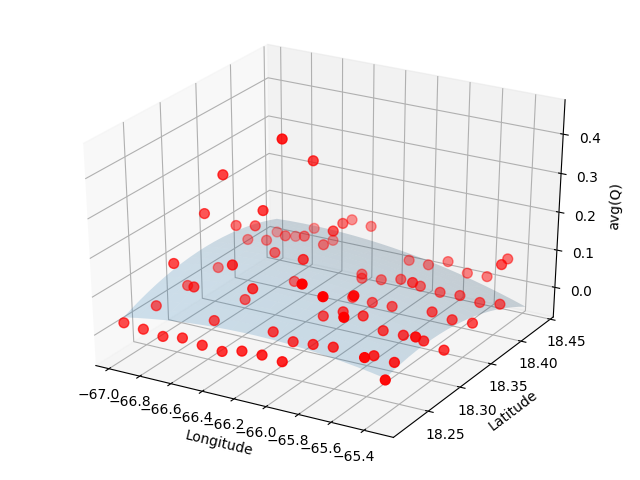
\includegraphics[width=0.76\textwidth, height=0.37\linewidth]{/home/vitowu/Documents/CourseMaterials/CourseMaterials/2018-2019_Term2/2019MCM-ProblemB/paper/container_1.png}
			}
			\caption[Simulation Result - Location of Container 1]
					{\tabular[t]{@{}l@{}}Simulation Result - Location of Container 1 \\ Fitting Surface: $f(x, y) = -1155.109 x - 1.9162y +  119.213xy - 0.2560 x^2 - 0.04972y^2$\endtabular}
		\end{figure}
			
			
		\begin{figure}[H]
			\centering
			\subfigure{}{
				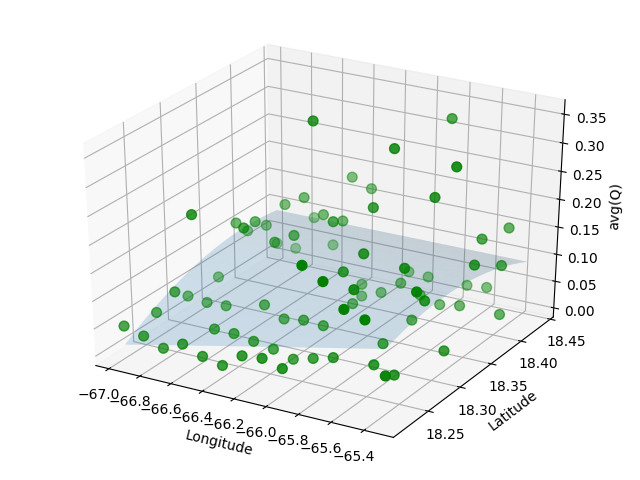
\includegraphics[width=0.82\textwidth, height=0.45\linewidth]{/home/vitowu/Documents/CourseMaterials/CourseMaterials/2018-2019_Term2/2019MCM-ProblemB/paper/container_2.png}
			}
			\caption[Simulation Result - Location of Container 2]
					{\tabular[t]{@{}l@{}}Simulation Result - Location of Container 1 \\ Fitting Surface: $f(x, y) =	-498.549 x +  4.921 y +  72.195 xy -0.27179 x^2  -0.0007 y^2$\endtabular}
		\end{figure}
			

		\begin{figure}[H]
			\centering
			\subfigure{}{
				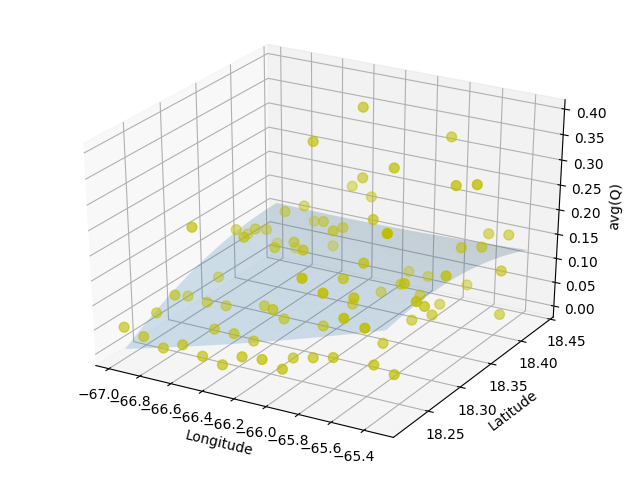
\includegraphics[width=0.82\textwidth, height=0.45\linewidth]{/home/vitowu/Documents/CourseMaterials/CourseMaterials/2018-2019_Term2/2019MCM-ProblemB/paper/container_3.png}
			}
			\caption[Simulation Result - Location of Container 3]	
					{\tabular[t]{@{}l@{}}Simulation Result - Location of Container 3 \\ Fitting Surface: $f(x, y) = -194.076 x +  8.613 y +  52.329xy- 0.4063 x^2+0.0084 y^2$\endtabular}
		\end{figure}
			
		From the regression plots we obtain that best three location to place the containers are: (18.36, -66.9), (18.37, -65.93) and (18.40, -66.01). The configurations of containers are listed in \textbf{Appendix}. In the simulation, the best result our model can get in average number of days are 87 in maximum.\par 
		Following map shows the exact location of three containers, in which the red marker denotes the first container, the yellow marker denotes the second container and the green marker denotes the last container.
		\begin{figure}[H]
			\centering
			\subfigure{}{
				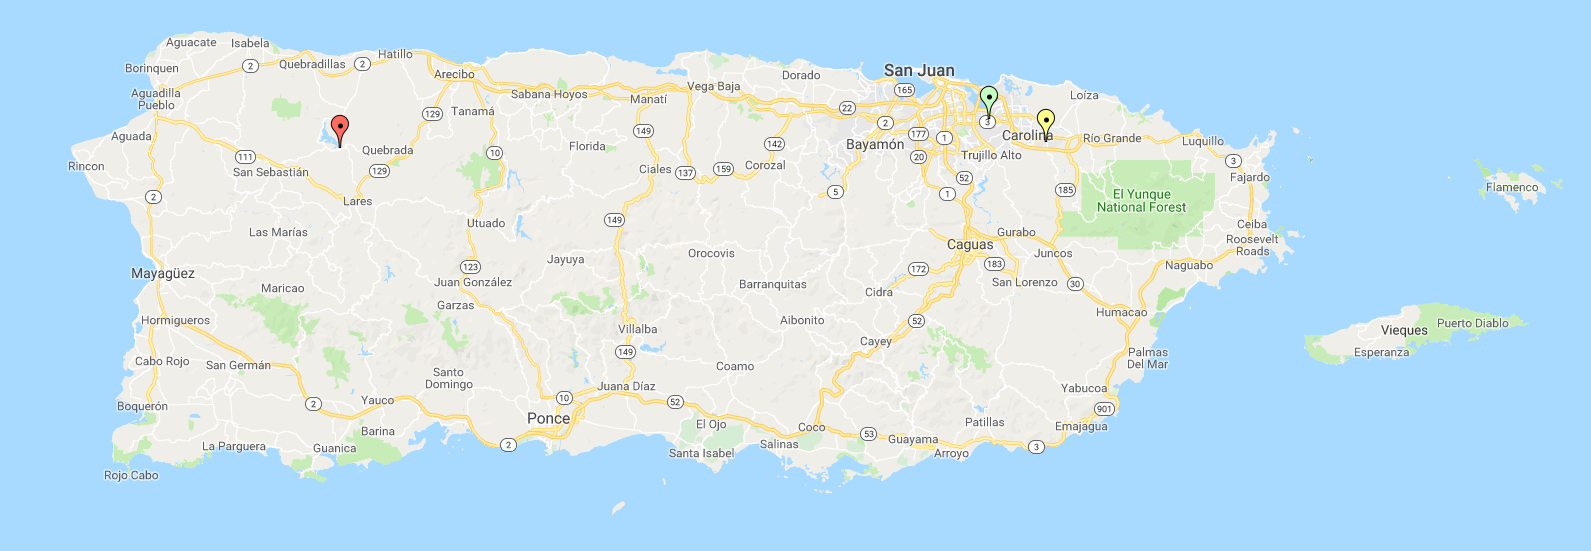
\includegraphics[width=0.95\textwidth]{/home/vitowu/Documents/CourseMaterials/CourseMaterials/2018-2019_Term2/2019MCM-ProblemB/paper/containers.png}
			}
		\end{figure}
	
	\section{Conclusion}
	In this paper, we provide models for cargo problem, drone flying strategy and the supply drop location. The cargo problem can be solved using dynamic optimization. The drone flying strategy and the container drop problem is the main problem in this paper. By using searching algorithm, dynamic programming, specifications of given cargoes and the consumption and geographical location of each hospital, we manage to find out the optimal solution under the preliminaries. The expected number of days that Puerto Rico can receive medical packages is 89 days, which is approximately to 3 months. According to media reports of Puerto Rico, over 90\% of main roads and infrastructures had been restored after 4 months, which validate our model as a reasonable model with compatibility to the real scenario. \par 
	
	However, our model gives little concern to the route discovering problem, which might also be very important in reality. Also, the model requires lots of power to finish its computation, which indicates that the model can be simplified.

	\section{Appendix. Memo for HELP, Inc}
	Our model gives 3-months medical support to Puerto Rico medical centers in maximum, and we have gives our solutions on how to pack the containers, where to settle the containers and how to route the drone. \par 
	However, the expectation of our model can achieved only if our assumptions in section \textbf{1.3} have been satisfied. Therefore, if you help us to meet our preliminary assumptions, we will sincerely appreciate it. \par 
	
	\section{Appendix. Container Configurations}	
	Here are optimal configurations we got from our model. \par 
	As what being proposed in section \textbf{1.5.1}, the optimal route of drones can be conclude from the saving algorithms if the configuration of container have been determined. Therefore, the route of drones are not necessary to be enumerated since we have given the exact container configurations. 
	\begin{figure}[H]
		\centering
		\subfigure{}{
			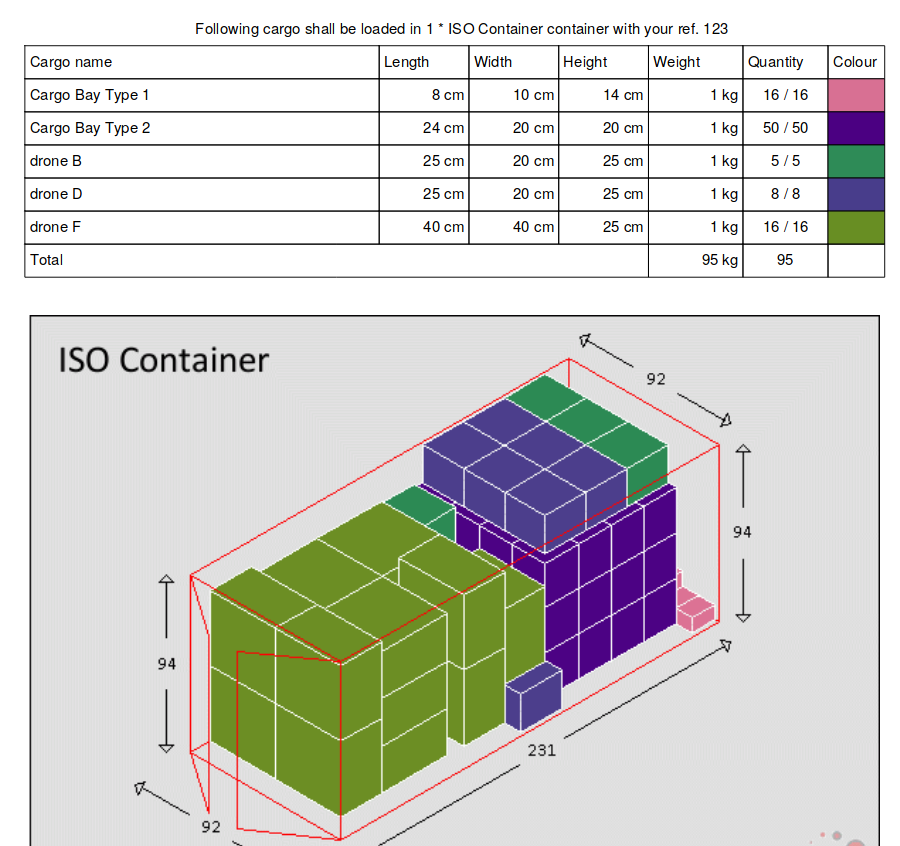
\includegraphics[width=0.75\textwidth,height=0.5\linewidth]{/home/vitowu/Documents/CourseMaterials/CourseMaterials/2018-2019_Term2/2019MCM-ProblemB/paper/container_conf1.png}
		}
		\caption{Simulation Result - Configuration of Container 1}
	\end{figure}
	
	
	\begin{figure}[H]
		\centering
		\subfigure{}{
			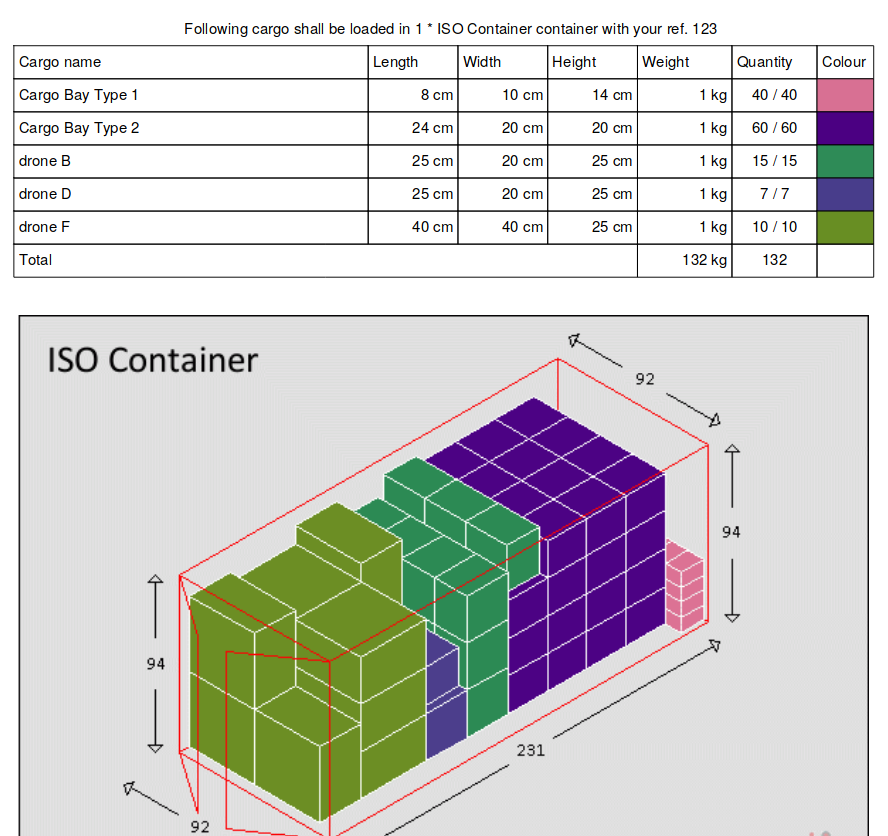
\includegraphics[width=0.75\textwidth,height=0.5\linewidth]{/home/vitowu/Documents/CourseMaterials/CourseMaterials/2018-2019_Term2/2019MCM-ProblemB/paper/container_conf3.png}
		}
		\caption{Simulation Result - Configuration of Container 2}
	\end{figure}
	
	
	\begin{figure}[H]
		\centering
		\subfigure{}{
			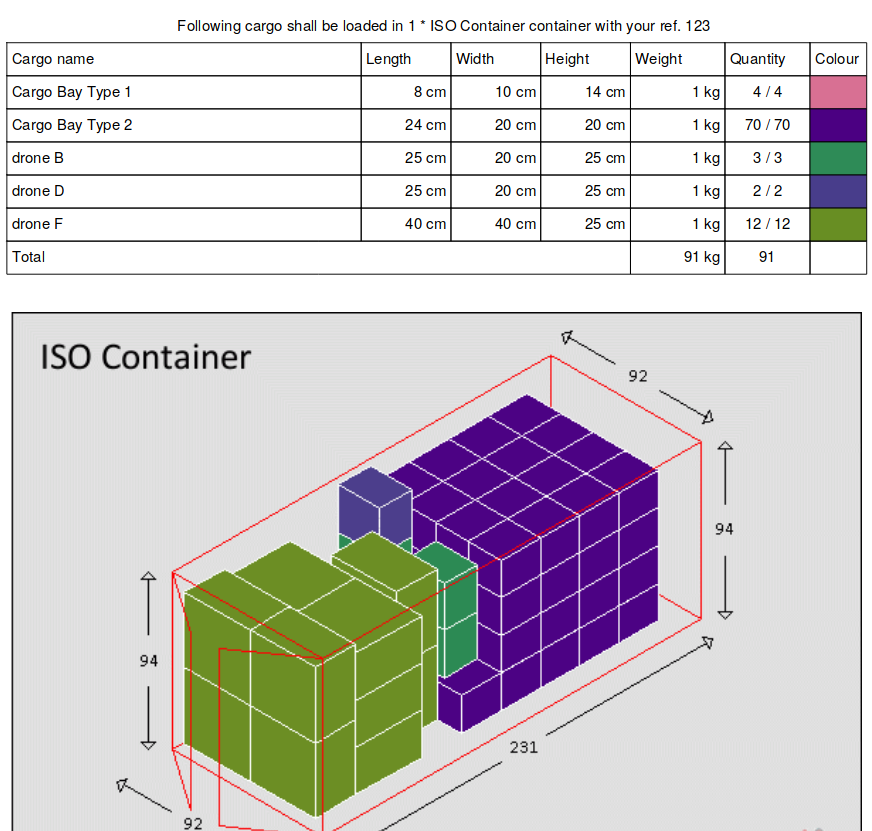
\includegraphics[width=0.75\textwidth,height=0.5\linewidth]{/home/vitowu/Documents/CourseMaterials/CourseMaterials/2018-2019_Term2/2019MCM-ProblemB/paper/container_conf2.png}
		}
		\caption{Simulation Result - Configuration of Container 3}
	\end{figure}
	
	\section{Appendix. Reference}
	\begin{thebibliography}{10}
		\bibitem{1}
		Karel Jeřábek, Peter Majercak, Tomas Kliestik, Katarina Valaskova.
		\textit{Application of Clark and Wright's Savings Algorithm Model to Solve Routing Problem in Supply Logistics}
		Naše more, 63(3)/2016., pp. 115-119
		
		\bibitem{2}
		Ariel E. Lugo, et.al. 
		\textit{Puerto Rican Karst - A Vital Resource}
		August, 2001
		
		\bibitem{3}
		Watson H. Monroe
		\textit{The Karst Landforms of Puerto Rico}
		Geological Survey professional paper ;899
		
		\bibitem{4}
		Oleg Granichin, Petr Skobelev, Alexander Lada, Igor Mayorov, Alexander Tsarev
		\textit{Cargo Transportation Models Analysis using Multi-Agent Adaptive Real-Time Truck Scheduling System}
		Proceedings of the 5th International Conference on Agents and Artificial Intelligence: Volume 2., pp.244-246
		
		\bibitem{5}
		Hui Dong, et.al.
		\textit{Emergency Operations Scheduling of Supply Chain Network in Disaster Reliefs}
		The State University of New Jersey., May, 2014
		
		\bibitem{6}
		Zengzhen Shao, Zujun Ma, Shulei Liu, Tongshuang Lv
		\textit{Optimization of a Traffic Control Scheme for a Post-Disaster Urban Road Network}
		Sustainability 2018, 10, 68.
		
		\bibitem{7}
		Warren B. Powell, Belgacem Bouzaiene-Ayari, Hugo P. Simao
		\textit{Dynamic Models for Freight Transportation}
		Department of Operations Research and Financial Engineering, Princeton University, September 14, 2005
		
		\bibitem{8}
		Ming Zhang, Jue Yu, Yifan Zhang and Hui Yu
		\textit{Programming Model of Emergency Scheduling with Combined Air-ground Transportation}
		Advances in Mechanical Engineering, 2017, Vol. 9(II) I-23
		
		\bibitem{9}
		Cejun Cao, Congdong Li, Qin Yang, Fanshun Zhang
		\textit{Multi-Objective Optimization Model of Emergency Organization Allocation for Sustainable Disaster Supply Chain}
		Sustainability 2017, 9, 2103
		
		\bibitem{10}
		Xiaowen Xiong, Fan Zhao, Yundou Wnag, Yapeng Wnag
		\textit{Research on the Model and Algorithm for Multi-modal Distribution of Emergency Supplies after Earthquake in the Perspective of Fairness}
		Hindawi, Mathematical Problems in Engineering, Volume 2019, Artical ID 1629321
		
	\end{thebibliography}
\end{document}